\section{Approach}
\label{sec:approach}
%the approach part mainly contains 3 parts: simplification, skip-thought language model and commonsense reasoning embedding

\begin{figure*}[htbp]
\centering
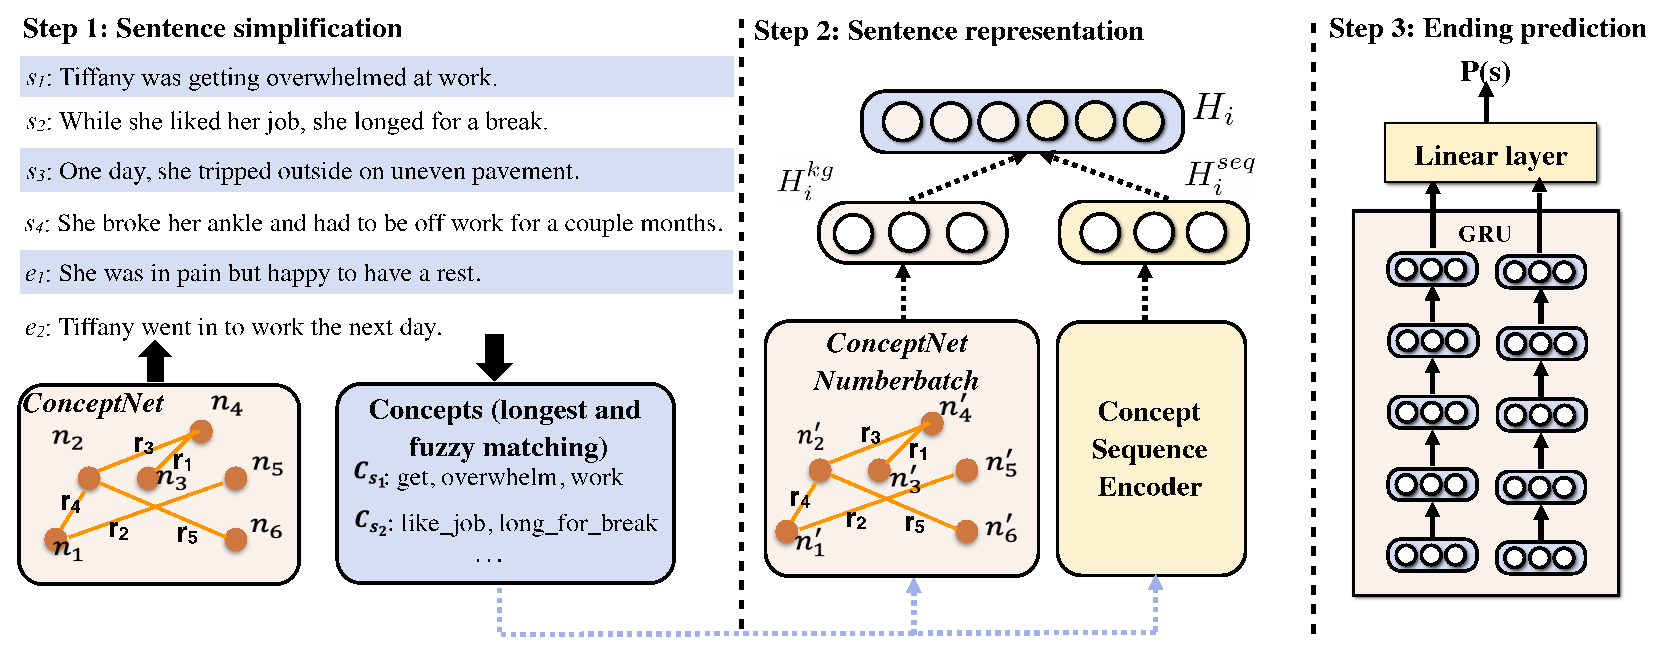
\includegraphics[width=1.8\columnwidth]{pictures/model}
\caption{Model overview: our model can be divided into three steps: sentence simplification, sentence representation and story classifier. ${n_1,...n_6}$ are the examples of token nodes in ConceptNet, ${r_1,...r_6}$  are the commonsense relations between the nodes. ${n_1^{'},...n_6^{'}}$ are the corresponding vector from Numberbatch which are trained on ConceptNet for main tokens.}\label{fig:model}
\end{figure*}

Given the story context $\textbf{s} = (s_1, s_2, ..., s_L)$ of $L$ sentences,
the target is to predict the correct ending from two candidate ending
sentences $e_1$ and $e_2$.
We propose to refine and extend story sentence representations
by incorporating commonsense knowledge from ConceptNet.
The model architecture is shown in \figref{fig:model}, which consists of three steps.
First, the model simplifies each story sentence, extracting commonsense related concepts.
%The first step is to extract the commonsense related knowledge with ConceptNet.
%It simplifies the sentences  simultaneously.
Second, the model constructs the sentence representation from two aspects:
the concept level encoding of the simplified sentence,
and its corresponding structured embeddings in ConceptNet.
% Second, we represent the tokens in a sentence in two aspects.
% One aspect is  an unsupervised language model. The encoder hidden state can be seen as the text sentence vector. The other aspect is the structured commonsense knowledge from ConceptNet. We take in the token representation form Numberbatch, which contains token embeddings pretrained on ConceptNet. Combining the representation of these two aspects, we obtain a better commonsense representation of a story sentences.
Finally, the model predicts the correct ending by applying a GRU based classifier.

\subsection{Sentence Simplification}
\label{sec:sentence simplification}



% Just as the story example in \figref{fig:story} , we can find some words in a sentence is  important for story understanding and story reasoning. In the five-sentence stories (context with right ending and context with wrong ending), \textit{getting overwhelmed at work} $\rightarrow$ \textit{liked job longed for break} $\rightarrow$\textit{One day tripped outside uneven pavement} $\rightarrow$ \textit{broke ankle off work for a couple months}$\rightarrow$\textit{pain happy rest} construct a coherent story in semantic level, and obviously, this knowledge chain is more reasonable than \textit{getting overwhelmed at work} $\rightarrow$ \textit{liked job longed for break} $\rightarrow$\textit{One day tripped outside uneven pavement} $\rightarrow$ \textit{broke ankle off work for a couple months}$\rightarrow$\textit{went in to work next day}. Although the sentences are not complete, we can still refer to the right ending of the story.


In order to extract the key concepts and events from a sentence
$s = \{w_1, ..., w_N\}$,
we use ConceptNet as the dictionary
and extract all the available concepts from $s$.
The output is a concept sequence $c_s = \{c_1, ..., c_M\}$
representing all mapped concepts within $s$.
The simplification process is described in \algoref{alg:simplify}.
As a preprocess step, we tokenize and lemmatize sentences with
NLTK~\cite{loper2002nltk} and Standford CoreNLP~\cite{manning2014stanford}.

For each concept $c$ in ConceptNet, let $|c|$ denote its word length.
If there exists a phrase $\{w_i, w_{i+1}, ..., w_{i+|c|}\}$ of $s$,
satisfying that $c$ is the subsequence of this phrase,
then $c$ is extracted and appended to $c_s$.
The length of the phrase equals to $|c|+1$,
so as to support a flexible matching.
For example, the concept ``broke ankle'' can be extracted
from the sentence ``broke her ankle''.
Afterwards, we remove duplicated concepts $c$ from $c_s$,
if it's strictly overlapped by other concepts in the sequence.
Finally, all kept concepts are sorted by their original positions
in the sentence.


% In order to choose the most important information from the sentence, we use ConceptNet token set  as a dictionary. Because it provides a large semantic graph which contains 1,500,000 nodes (concepts) and millions of edges for English. Its knowledge is collected from many sources that include expert-created resources, crowd-sourcing, and games with a purpose. We assume the tokens that appear in ConceptNet are important for commonsense understanding and reasoning.

% We use longest and fuzzy match for each sentence with the ~\algoref{alg:simplify}. We construct a dictionary which grouped by the first word of concepts. The keys are the first words. The values for each key are the concepts starting with the same dictionary key word. For the preliminary work, we tokenize and lemmatize sentence with NLTK and Standford’s CoreNLP tools ~\cite{manning2014stanford}. When traversing every word in a sentence, we choose the longest token. We also allow a discontinuous placeholder for fuzzy match. For example,  ``break'' in sentence ``She broke her ankle and had to be off work for a couple months''  should not be exactly matched with ``break ankle''  from dictionary. With the placeholder, we search extra one  continuous word in the sentence and will find this token belongs to the sentence. We can extract  ``broke ankle'' and  ``for couple months'' for this sentence. With this matching method, we can simplify a sentence $s_i$ in story $\textbf{s}$ to a token set. Let $c_{s_i} = c_{s_i}^{1},...,c_{s_i}^{D}$ be the $i_{th}$ sentence in all the serialized story sequence, where $D$ is the number of tokens matched in ConceptNet.

\begin{algorithm}[tb]
\small
\caption{Simplification algorithm}
\label{alg:simplify}
\textbf{Input}: ConceptNet $C$, sentence $s=\{w_1, ..., w_N\}$\\
\textbf{Output}: Concept sequence $c_s=\{c_1, ..., c_M\}$
\begin{algorithmic}[1] %[1] enables line numbers
  % \Procedure{Simplify}{$C, S$}
  %   \STATE{$D$ \gets $xxx$}
  %   \FOR {Concept $c$ in $C$}
  %     \STATE{xxx}
  %   \ENDFOR
  % \EndProcedure
% \STATE Construct a dictionary $D$
% \FOR{token $x$ in ConceptNet nodes}
% \STATE $D[x.headword]$.append$(x)$
% \ENDFOR
% \STATE key token set $c_i = [$ $]$
% \FOR{index $j$, word $w$ in sentence $s_i$}
% \FOR {token $d$ in alternative token set $D[w]$}
% \IF{words in $d$ is the subset of $s_{i}[j:j+d.length+2]$}
% \STATE $c_i$.append($d$)
% \ENDIF
% \ENDFOR
% \ENDFOR
% \FOR{index $k$, token $t$ in $c_i.sortbylength()$}
% \IF {words in $c_i$ is the subset of any token in $c_{i}[k:]$}
% \STATE $c_i$.del($t$)
% \ENDIF
% \ENDFOR
% \STATE \textbf{return}  $c_i$
\Procedure{Simplify}{$C, s$}
  \State {$c_s \gets \{\}$}
  \For {$c \in C$}
    \For {$w_i \in s$}
      \If {$c ~\textrm{is a subsequence of}~ \{w_i, w_{i+1}, ..., w_{i+|c|}\}$}
        \State {$c_s \gets c_s + \{c\}$}
      \EndIf
    \EndFor
  \EndFor
  \State {$c_s \gets DupConceptFilter(c_s)$}
  \State {$c_s \gets SortByOrder(c_s)$}
  \State \textbf{return} {$c_s$}
  \EndProcedure
\end{algorithmic}
\end{algorithm}

\subsection{Sentence Representation}
\label{sec:represent}
The sentence representation consists of two parts:
concept sequence representation and structured knowledge representation.

\subsection*{Concept Sequence Representation}

After simplification process, the concept sequence of a sentence
is encoded into vector representation using a sequential encoder.
In order to reduce the vocabulary size of the encoder,
the concept sequence $c_s$ is converted into a flatten word sequence $s'$,
which is the concatenation of the names of all the concepts in $c_s$.
Compared with the original sentence, $s'$ a simplified word sequence
where commonsense-irrelevant information are discarded.

We adopt GRU as the sequential encoder in our model,
which produces a hidden state $h_t$ of $t$-th word in $s'$.
The concept sequence embedding $H^{seq}$ is calculated
as follows:
% which produces a hidden state $h_{i}^{t}$ at each time step. $h_{i}^{D}$ can represent the whole sentence. Following ~\citeauthor{kiros2015skip} 's work, we iterate the following equations of GRU to encode all tokens in a sentence:
\begin{equation}
\begin{aligned}
  z_{t} & =\sigma\big(x_{t}U_{z}+h_{t-1}W_{z}\big), \\
  r_{t} & =\sigma\big(x_{t}U_{r}+h_{t-1}W_{r}\big), \\
  \tilde{h}_{t} & =\tanh\big(x_{t}U_{h}+(r_{t}\ast h_{t-1})W_{h}\big), \\
  h_{t} & =(1-z_{t})\ast h_{t-1}+z_{t}\ast\tilde{h}_{t}, \\
        & H^{seq} = h_{-1},
\end{aligned}
\end{equation}
\noindent
where $r_{t} $ is the reset gate,
$z_{t}$ is the update gate,
$\ast$ denotes a element-wise product,
and $h_{-1}$ is the last hidden state of $s'$.
$U_{z},U_{r},U_{h},W_{z}, W_{r}, W_{h}$ are matrix to be trained.

Pre-train models are widely used in existing works.
For better capturing the inter-sentence semantic relationship,
we pre-train the concept sequence encoder using Skip-thought model~\cite{kiros2015skip}.
The training data of Skip-thought consists of 3-tuples
($s_{i-1}', s_i', s_{i+1}'$), which are simplified sentence tri-grams
collected from various unlabeled stories.
The objective of the pre-train model is the sum of the log-probabilities
of predicting both the previous and next sentence given $s_i'$.


% we pretrain our
% sentence representation model on approximate 100,000
% ROCStories ~\cite{mostafazadeh2016story}  (five-sentence stories where
% the 5th sentence is the correct ending).

% By the strong advantage of
% simplification which reduces unrelated knowledge for commonsense reasoning
% in a sentence. We can train a better model within less data
% (See \secref{sec:result}). Let original story $\textbf{s}=(s_1, s_2, s_3, s_4, s_5)$, where $s_i$ is a sentence.



% Given a sequence tuple ($s_{i-1}, s_i, s_{i+1}$) we can get a token tuple ($c_{s_{i-1}}, c_{s_i}, c_{s_{i+1}}$).

% There are two decoder in this language model. Both of the decoders condition on the encoder hidden state $h_{i}^{D}$, and still use GRU structure. The target outputs for each decoders are $c_{i-1}$ and $c_{i+1}$. The objective optimized is the sum of the log-probabilities for the forward and backward tokens conditioned on the encoder representation.

\subsection*{Structured Knowledge Representation}

Previous study~\cite{chen2018incorporating} has shown that
structured knowledge in ConceptNet can take external knowledge to
complete the commonsense reasoning in stories.
Different from the existing research,
rather than generating handcrafted features,
we expected to incorporate the structured commonsense knowledge
in sentence representation.
Numberbatch\footnote{\url{https://github.com/commonsense/conceptnet-numberbatch}}
is the pre-trained concept embedding with ConceptNet knowledge graph,
which contains more than 2,000,000 popular concepts.
Given the concept sequence $c_s = \{c_1, ..., c_M\}$,
we define the structured knowledge representation $H^{kg}$
as the summation of each concept:
\begin{equation}
  H^{kg} = \sum_{c \in c_s}{Numberbatch(c)},
\end{equation}
\noindent
where $Numberbatch(\cdot)$ returns the concept vector.
If one concept is not in Numberbatch, we approximate its concept vector
by averaging all vectors of its words in Numberbatch.

% We have
% the token set $c_{s_i}=(c_{s_i}^{1},...,c_{s_i}^{D})$ for sentence $s_i$, and we use ~\eqref{eq:sum} to compute structured representation for  $s_i$. Each token in $c_{s_i}$ should have a 300 dimension corresponding representation (${c_{s_i}^{1}}',...,{c_{s_i}^{D'}}')$ in Numberbatch. If the token isn't in Numberbatch, and it consist of several words. We will give this token an vector representation by average all the word vectors in Numberbatch. We will sign a 300 dimension zero vector for the word that can not be find in Numberbatch. Getting the representation for every token in $c_{s_i}$, the structured sentence representation for $s_i$ can be denoted as $o_i$, a 300 dimension vector summed up by each token vector.
%
%
% \begin{equation}
% \begin{aligned}
%     o_{l} & = Sum({c_{s_i}^d}'),d\in \big[1,D\big]  \label{eq:sum}
% \end{aligned}
% \end{equation}

\subsection{Ending Prediction}
\label{sec:classifier}

Given the pre-trained concept sequence encoder and
Numberbatch concept embedding,
% We have the pretrained parameters from the sequence text model and Numberbatch. Our sentence representation can be combined with these two parts.
the representation of the $i$-th sentence $s_i$ is defined as
the concatenation of two components: $H_i=[H_i^{seq}; H_i^{kg}]$.
For predicting the correct ending from two candidates,
% In order to predict which ending is more consistent to the story context,
we separately bind the two candidate endings to the context sentences,
and apply a simple GRU classifier to judge
which 5-sentence story $(s_1, s_2, s_3, s_4, e)$
is more likely to be correct:
\begin{equation}
  \begin{aligned}
  & Q_l = Dropout(GRU(Q_{l-1}, H_l)), l \in [1, 5], \\
  & P(y|s_1, s_2, s_3, s_4, e) = softmax(W_{out} Q_5 + b_{out}),
\end{aligned}
\end{equation}
where $y \in \{0, 1\}$ is the label indicating whether $e$ is the
correct ending, and $Q_l$ is the hidden state of the $l$-th sentence.
$Dropout$ layer is applied to avoid overfitting.
% So, the probability of $e_{i}$ being the correct ending:
% \begin{equation}
% \begin{aligned}
%     P\big(y | s_1, s_2, s_3, s_4, e_i\big) &= P\big(s\big)
% \end{aligned}
% \end{equation}
